\documentclass[handout]{beamer}
\usepackage{textpos}
\usepackage{listings}
\usepackage{hyperref}

\usepackage{caption}
\captionsetup[table]{labelformat=empty}

\usepackage{xcolor}
\definecolor{mygreen}{rgb}{0,0.6,0}
\definecolor{mygray}{rgb}{0.5,0.5,0.5}

\usepackage{graphicx}% http://ctan.org/pkg/graphicx
\usepackage{booktabs}

\lstset{language=C++,
           basicstyle=\ttfamily\scriptsize,
           keywordstyle=\color{blue}\ttfamily,
           stringstyle=\color{red}\ttfamily,
           commentstyle=\color{mygreen}\ttfamily,
          breaklines=true,
          captionpos=b,
          numbers=left,
          numbersep=5pt,
          numberstyle=\tiny\color{mygray},
          rulecolor=\color{black},
          xleftmargin=\parindent,
          frame=single,
          backgroundcolor=\color{white}
}

%\hypersetup{%
%colorlinks=true,% hyperlinks will be black
%linkcolor=blue
%}

% \usepackage{beamerthemesplit} // Activate for custom appearance

\setbeamercolor{normal text}{fg=black,bg=white}
\definecolor{beamer@blendedblue}{rgb}{0,0,0}
\setbeamercolor{structure}{fg=beamer@blendedblue}


\title{CUDA Fundementals}
\author{
	\includegraphics[width=3cm]{../media/logo/NVLogo_2D.eps}
	\vspace{0.75cm}
	\\}
\date{\today}

\begin{document}

\frame{\titlepage}

%\section[Outline]{}
\begin{frame}{Outline}
\tableofcontents
\end{frame}

\addtobeamertemplate{frametitle}{}{%
\begin{textblock*}{200mm}(.75\textwidth,-0.35cm)
\includegraphics[width=3cm]{../media/logo/NVLogo_2D_H.eps}
\end{textblock*}}

\addtobeamertemplate{navigation symbols}{}{%
    \usebeamerfont{footline}%
    \usebeamercolor[fg]{footline}%
    \hspace{1em}%
    \insertframenumber/\inserttotalframenumber
}


\section{SIMD Programing Paradigm}
\begin{frame}{Parallel Algorithms in SIMD}
\begin{itemize}
\itemsep1em
\setbeamercovered{transparent}
	\item<1->Recall that GPU hardware is designed for maximizing thread execution throughput.
	\item<1->And, this throughput-oriented design is effective since all the GPU threads are working a single CUDA kernel in parallel.
	\item<1->Each GPU thread execute the same kernel.  Once each individual thread has finished sequentially executing the kernel code, the kernel task as a whole is complete.  
	\item<1->That is, each thread executes the same kernel but on it's own chunk or piece of the data.  This style of programing is called \emph{single instruction multiple data} (SIMD) pronounced ``sim-dee''
\end{itemize}
\end{frame}

\begin{frame}{Parallel Algorithms in SIMD}
\begin{itemize}
\setbeamercovered{transparent}
	\item<1->In SIMD, each thread executes the same kernel but only on it's own small piece of the data.
	\item<1->Each thread must have some kind of index information to provide context for which piece of the data to work on.
	\item<1->Threads in SIMD use there own index info as a key to determine which data to access.
	\item<1->This means that in massively parallel SIMD algorithms, thread organization plays a very important role.
	\item<1->Kernel thread organization will typically closely mirror the data dimensions so that thread index is aligned with data index.  
\end{itemize}
\end{frame}

\section{Vector Addition Example}
\begin{frame}{Vector Addition Definition}
\begin{itemize}
\itemsep1em
	\item<1>Suppose we have two vectors of type double with matching dimensions: $\textbf{a}$ and $\textbf{b}$ both of size $1\times N$
	\item<1>Our goal is to create a resultant vector $\textbf{c}$ of doubles having size $1\times N$ where $\textbf{c}[i] = \textbf{a}[i]+\textbf{b}[i]$ 
	\item<1>Using a traditional sequential programing approach a simple {\fontfamily{qcr}\selectfont for}-loop would solve this nicely:
\end{itemize}

\end{frame}


\begin{frame}[fragile]{Traditional Vector Addition in C}
\lstinputlisting[language=C++,caption={Vanilla vector addition in C}]{../src/vecAdd.c}
\end{frame}

\begin{frame}{Embarrassingly Parallel Problems}
\begin{itemize}
\itemsep1em
	\item<1->Vector addition, as defined, makes a good initial parallel programing exercise since each element of the output vector {\fontfamily{qcr}\selectfont \textbf{c}} can be computed independent of all other elements. 
	\item<1->Problems (or algorithms) which exhibit perfect data parallelism, such as vector addition, are called \emph{embarrassingly parallel}.
	\item<1->Launching a CUDA kernel typically generates a large number of threads to exploit data parallelism. 
\end{itemize}
\end{frame}

\begin{frame}[fragile]{SIMD Vector Addition with CUDA}
\begin{lstlisting}[caption={A SIMD example for vector addition using CUDA}]
#define N 256

// Kernel definition (i.e. device code executed on the GPU)
__global__ void VecAdd(float* a, float* b, float* c){

    // get local thread context
    int i = threadIdx.x;
    
    // perform operation on data
    c[i] = a[i] + b[i];
}
// host code executed by the CPU
int main(){
    ...
    // launch configuration
    dim3 gridSize (1,1,1), blockSize(N,1,1);
    
    // kernel launch
    VecAdd<<<gridSize, blockSize>>>(a, b, c);
    ...
}
\end{lstlisting}
\end{frame}

\begin{frame}{SIMD Vector Addition Visualization}
\begin{figure}
\begin{center}
\includegraphics[width=5.5cm]{../media/vector_add_cuda.pdf}
\caption{Thread visualization of vector addition CUDA kernel.  Here thread0 calculates {\fontfamily{qcr}\selectfont \textbf{c}[0]}, thread1 calculates {\fontfamily{qcr}\selectfont \textbf{c}[1]}, and so on.  Each thread performs the same set of operations, but on its own piece of data.}
\end{center}
\end{figure}
\end{frame}


\begin{frame}{Kernel Launch Thread Configurations}
\centering

\begin{table} 
\resizebox{\linewidth}{!}{
\begin{tabular}{ | c | c | c | c | c | c | c | c | c | c | c | c | c | c | c | c | c | c | c | c | c | c | c | c | c | c | c | c | c | c | c | c |}
\hline
  0 & 1 & 2 & 3 & 4 & 5  & 6 & 7 & 8 & 9 & 10 &11 & 12 & 13 & 14 & 15 & 16 & 17 & 18 & 19 & 20 & 21  & 22 & 23 & 24 & 25 & 26 & 27 & 28 & 29 & 30 & 31  \\ 
\hline
\end{tabular} 
}
\caption{{\fontfamily{qcr}\selectfont dim3 blockSize(32,1,1)}}
\end{table} 

\begin{table} 
\resizebox{\linewidth}{!}{
\begin{tabular}{ | c | c | c | c | c | c | c | c | c | c | c | c | c | c | c | c | c | c | c | c | c | c | c | c | c | c | c | c | c | c | c | c |}
\hline
  0 & 1 & 2 & 3 & 4 & 5  & 6 & 7 & 8 & 9 & 10 &11 & 12 & 13 & 14 & 15   \\  
\hline
 16 & 17 & 18 & 19 & 20 & 21  & 22 & 23 & 24 & 25 & 26 & 27 & 28 & 29 & 30 & 31 \\
\hline
\end{tabular} 
}
\caption{{\fontfamily{qcr}\selectfont dim3 blockSize(16,2,1)}}
\end{table} 

\begin{table} `
\resizebox{!}{!}{
\begin{tabular}{ | c | c | c | c | c | c | c | c |}
\hline
  0 & 1 & 2 & 3 & 4 & 5  & 6 & 7  \\  
\hline
  8 & 9 & 10 &11 & 12 & 13 & 14 & 15 \\
\hline
 16 & 17 & 18 & 19 & 20 & 21  & 22 & 23  \\
\hline
  24 & 25 & 26 & 27 & 28 & 29 & 30 & 31 \\
\hline
\end{tabular} 
}
\caption{{\fontfamily{qcr}\selectfont dim3 blockSize(8,4,1)}}
\end{table} 

\end{frame}

\begin{frame}{Kernel Thread Organization}
\centering
\begin{figure}
\label{fig:gridorg}
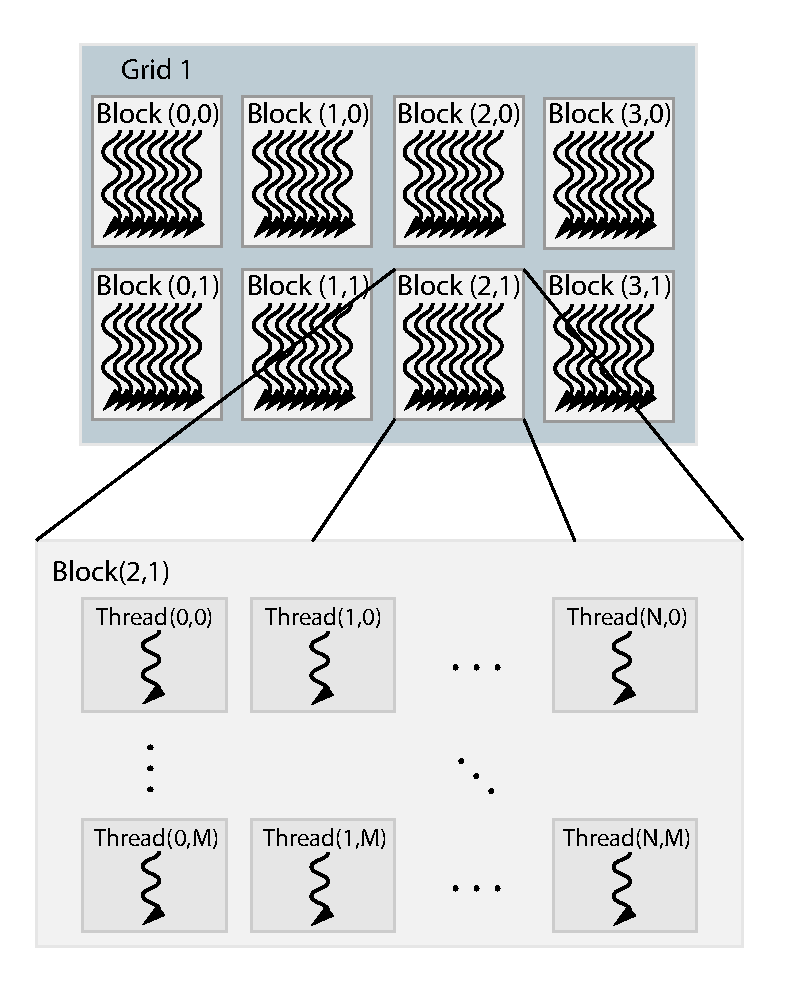
\includegraphics[width=5.5cm]{../media/grid_org.pdf}
\caption{dim3 gridSize(4,2,1) with dim3 blockSize(N,M,1).}
\end{figure}
\end{frame}

\begin{frame}{Kernel Thread Configurations}
\begin{itemize}
	\item<1->Grids can have up to 65535x65535 blocks on SM 1.x and 65535x65535x65535 blocks with SM 2.x hardware.
	\item<1->Thread-blocks are further divided into \href{http://docs.nvidia.com/cuda/cuda-c-programming-guide/index.html\#simt-architecture}{\color{blue}\emph{warps}} of 32 threads.  
	\item<1->A warp is the fundamental unit of granularity on the SM.
	\item<1->Therefore, thread-block size should be specified modulo 32.
	\item<1->Special read-only registers give each \href{http://docs.nvidia.com/cuda/cuda-c-programming-guide/index.html\#thread-hierarchy}{\color{blue}thread context} via built-in variables \emph{threadIdx}, \emph{blockIdx}, \emph{gridDim} and \emph{blockDim}.
	\item<1->Taken together these variables can be used to compute which part of a problem the thread will operate on.
	\item<1->Note that there is no performance benefit with 2D or 3D blocks and grids, but they often match better to the data organization.
\end{itemize}
\end{frame}

%\begin{frame}{A Note on CUDA Header Files}
%\begin{itemize}
%\itemsep1em
%	\item<1->{There are three key header files when programing in CUDA:}
%	\break
%	\begin{itemize}
%	\itemsep1em
%		\item<1->{\fontfamily{qcr}\selectfont cuda.h} defining types and host functions for the CUDA \emph{driver} API.
%		\item<1->{\fontfamily{qcr}\selectfont cuda\_runtime\_api.h} which defines types and host functions and types for the CUDA \emph{runtime} API. 
%		\item<1->{\fontfamily{qcr}\selectfont cuda\_runtime.h} contains a superset of definitions including everything from {\fontfamily{qcr}\selectfont cuda\_runtime\_api.h}, as well as built-in type definitions, function overlays for the CUDA language extensions, and device intrinsic functions.
%	\end{itemize}
%	\item<1->Notice that when compiling with \textbf{{\fontfamily{qcr}\selectfont nvcc}} the appropriate CUDA headers are included automatically.
%\end{itemize}
%
%\end{frame}

\begin{frame}{Understanding CUDA Kernel Signatures}
\begin{itemize}
\itemsep1em
	\item<1->A kernel function \emph{must} have a {\fontfamily{qcr}\selectfont void} return type.
	\item<1-> There are three kernel function type qualifiers which signal \textbf{{\fontfamily{qcr}\selectfont nvcc}} for how the function should be compiled:
	\begin{itemize}
	\itemsep1em
		\item<1->{\fontfamily{qcr}\selectfont \_\_global\_\_} says that the function will be \emph{executed} on the device (i.e. it's a kernel) but callable (launched) from the host.
		\item<1->{\fontfamily{qcr}\selectfont \_\_device\_\_} also says that the function will be executed on the device but is \emph{only callable from the device}.  Think kernel helper functions here.
		\item<1->Finally, {\fontfamily{qcr}\selectfont \_\_host\_\_} tells \textbf{{\fontfamily{qcr}\selectfont nvcc}} that this function will only be executable and callable from the host (i.e. this is just a regular C function!).
	\end{itemize}
\end{itemize}
\end{frame}

\begin{frame}{Kernel Restrictions}
There are a few kernel coding restrictions to keep in mind:
\break
\begin{itemize}
\itemsep1em
	\item<1->Kernel functions can \emph{only} access device memory\footnote{Exception when using \emph{mapped pinned memory} (more later)\hfill\break}
	\item<1->Again, kernel functions must have {\fontfamily{qcr}\selectfont void} return type
	\item<1->No support for variable number of arguments
	\item<1->No support for static variables
	\item<1->No support for function pointers
	\item<1->Exhibit asynchronous behavior
\end{itemize}
\end{frame}

\begin{frame}[fragile]{Kernel Launch Runtime Syntax}
When using the CUDA runtime API, the generic kernel launch triple-angle-bracket syntax is:
\hfill\break
\begin{lstlisting}[caption={Kernel launch syntax using runtime API}]
KERNEL<<<gridSize, blockSize, sharedMem, stream>>>(args)
\end{lstlisting}
\begin{itemize}
	\item<1->{\fontfamily{qcr}\selectfont KERNEL} specifies the kernel function to launch
	\item<1->{\fontfamily{qcr}\selectfont gridSize} specified the number of thread-blocks in the form of a {\fontfamily{qcr}\selectfont dim3} structure
	\item<1->{\fontfamily{qcr}\selectfont blockSize} specifies the size of each thread-block in three dimensions as a {\fontfamily{qcr}\selectfont dim3}.
	\item<1->{\fontfamily{qcr}\selectfont sharedMem} specifies the amound of additional shared memory to reserve for each thread-block. Default: 0
	\item<1->{\fontfamily{qcr}\selectfont stream} specifies the logical execution queue for the kernel
\end{itemize}
\end{frame}

\begin{frame}[fragile]{{\fontfamily{qcr}\selectfont dim3} Structure}
The {\fontfamily{qcr}\selectfont dim3} structure is used to specify the grid and thread-block sizes and has 3 members ({\fontfamily{qcr}\selectfont x}, {\fontfamily{qcr}\selectfont y}, and {\fontfamily{qcr}\selectfont z}) with a default constructor which initializes {\fontfamily{qcr}\selectfont y} and {\fontfamily{qcr}\selectfont z} to 1.
\begin{lstlisting}[caption={{\fontfamily{qcr}\selectfont dim3} structure definition defined in {\fontfamily{qcr}\selectfont vector\_types.h}}]
struct __device_builtin__ dim3
{
    unsigned int x, y, z;
#if defined(__cplusplus)
    __host__ __device__ dim3(
    unsigned int vx = 1,
    unsigned int vy = 1,
    unsigned int vz = 1) : x(vx), y(vy), z(vz) {}
    __host__ __device__ dim3(uint3 v):x(v.x),y(v.y),z(v.z){}
    __host__ __device__ operator uint3(void){
        uint3 t;  t.x = x;   t.y = y;  t.z = z;  return t;
    }
#endif
};
\end{lstlisting}
\end{frame}

\begin{frame}[fragile]{Kernel Launch with Driver API}
Kernels can be launched from the CUDA driver API using the {\fontfamily{qcr}\selectfont cuLaunchKernel()} call 
\begin{lstlisting}[caption={{\fontfamily{qcr}\selectfont cuLaunchKernel()} in the CUDA driver API}]
CUresult CUDAAPI cuLaunchKernel(
    CUfunction f,
    unsigned int gridDimX,
    unsigned int gridDimY,
    unsigned int gridDimZ,
    unsigned int blockDimX,
    unsigned int blockDimY,
    unsigned int blockDimZ,
    unsigned int sharedMemBytes,
    CUstream hStream,
    void **kernelParams,
    void **extra
);
\end{lstlisting}
\end{frame}

\begin{frame}[fragile]{Kernel Launch with Driver API}
However, note that kernel launches using the runtime API get translated into even lower driver API calls using {\fontfamily{qcr}\selectfont cudaLaunch()}, {\fontfamily{qcr}\selectfont cudaConfigureCall()}, {\fontfamily{qcr}\selectfont cudaSetupArgument()}.  For example, the {\fontfamily{qcr}\selectfont VecAdd} kernel launch
\begin{lstlisting}
VecAdd<<<1, N>>>(a, b, c);
\end{lstlisting}
generates ({\fontfamily{qcr}\selectfont vecAdd.cudafe1.stub.c}, using {\fontfamily{qcr}\selectfont nvcc} {\fontfamily{qcr}\selectfont --keep})
\begin{lstlisting}[]
void __device_stub__Z6vecAddPfS_S_(
    float *__par0, 
    float *__par1, 
    float *__par2)
{
        __cudaSetupArgSimple(__par0,  0UL);
        __cudaSetupArgSimple(__par1,  8UL);
        __cudaSetupArgSimple(__par2, 16UL);
        __cudaLaunch(
            ((char *)((void ( *)(float *, float *, float *))vecAdd))
        );
}
\end{lstlisting}
\end{frame}


\begin{frame}{{\fontfamily{qcr}\selectfont C++} Class Restrictions}
All {\fontfamily{qcr}\selectfont C++} classes participating in a kernel launch must be ``plain old data'' (POD) with the following characteristics:
\hfill\break
\begin{itemize}
\itemsep1em
	\item<1->No user-declared constructors or destructors
	\item<1->No user-defined copy assignment operator
	\item<1->No non-static data members that are not themselves POD
	\item<1->No private or protected non-static data
	\item<1->No virtual functions or base classes
\end{itemize}
\hfill \break
Classes that violate these rules my be used in CUDA, or even in CUDA kernels; they simply cannot be used for kernel launch.
\end{frame}


\begin{frame}{Kernel Execution}
\begin{itemize}
	\item<1->Once a kernel is launched, it runs as a \emph{grid} of \emph{blocks} of \emph{threads}.
	\item<1->Each thread block is assigned to a streaming multiprocessor (SM) on the device.
	\item<1->Not all thread blocks run concurrently, necessarily.
	\item<1->The CUDA programming model makes \emph{no guarantees whatsoever as to the order of execution} or whether certain blocks or threads can run concurrently.
	\item<1->Again, CUDA developers can never assume that all the threads in a kernel launch are executing concurrently.
	\item<1->It is easy to launch a kernel with more threads than the device can hold and therefore some will not start executing until others have finished.
\end{itemize}
\end{frame}

%\begin{frame}{Kernel Execution Continued}
%\begin{itemize}
%	\item<1->Thread-blocks are further divided into \emph{warps} of 32 threads.  
%	\item<1->Each thread in a warp is called a \emph{lane}.
%	\item<1->A warp is the fundamental unit of granularity on the SM.
%	\item<1->Grids can have up to 65535x65535 blocks on SM 1.x and 65535x65535x65535 blocks with SM 2.x hardware.
%	\item<1->Thread-blocks do not move from SM to SM.  A thread-block resides on an SM for the lifetime of the kernel.
%	\item<1->There can be many active warps from different blocks at the same time on a single SM. 
%	\item<1->Warp schedulers dispatch instructions as requested resources become available.
%	\item<1->All 32 threads execute the same instruction, each thread using its own set of registers to perform the requested operation.
%\end{itemize}
%\end{frame}

\begin{frame}{Asynchronous Error Handling}
\begin{itemize}
	\item<1->Kernel launches are \emph{asynchronous}.
	\item<1->As soon as a kernel is submitted to the hardware, it begins executing in parallel with the CPU.
	\item<1->On most platforms, the kernel will start executing on the GPU microseconds after the CPU has finished processing the launch command\footnote{With the Windows Display Driver Model (WDDM), it may take longer to launch a kernel because the driver must perform an OS \href{https://msdn.microsoft.com/en-us/library/windows/hardware/ff565689(v=vs.85).aspx}{\color{blue}kernel thunk} in order to submit the launch to the hardware.\hfill\break}.
	\item<1->If the kernel encounters an error (e.g. invalid memory access, etc), the error is reported to the driver (and the application) some time after the kernel launch.  
	\item<1->The best way to check for such errors is to synchronize with the GPU using {\fontfamily{qcr}\selectfont cudaDeviceSynchronize()} or {\fontfamily{qcr}\selectfont cuCtxSynchronize()}
\end{itemize}
\end{frame}

\begin{frame}[fragile]{Error Handling Continued}
\begin{itemize}
	\item<1->Most CUDA runtime API calls return type {\fontfamily{qcr}\selectfont cudaError\_t}
	\item<1->It is standard practice to define error-handling macro to wrap API calls.  For example
\end{itemize}
\begin{lstlisting}[caption={Error handling macro for CUDA}]
#include <cuda_runtime.h>
#define CHECK(call)
{
    const cudaError_t error = call;
    if (error != cudaSuccess){
        printf("Error: %s:%d",__FILE__,__LINE__);
        printf("code:%d, reason: %s\n", error, cudaGetErrorString(error));
        exit(1);
    }
}
\end{lstlisting}
\end{frame}

\begin{frame}[fragile]{Error Handling Continued}
\begin{itemize}
\itemsep1em
	\item<1->The error-handling macro can be use around {\fontfamily{qcr}\selectfont cudaDeviceSynchronize()} after a kernel invocation to check for kernel errors
	\item<1->If an error in the kernel execution has occurred, the error string "unspecified launch failure" is returned.
\end{itemize}
\begin{lstlisting}[caption={Catching kernel failures with CHECK macro}]
    kernel_function<<<gridsz,blocksz>>>(args);
    CHECK(cudaDeviceSynchronize());
\end{lstlisting}
\begin{itemize}
	\item<1->See also: {\fontfamily{qcr}\selectfont cudaGetLastError()}
\end{itemize}
\end{frame}

\begin{frame}{Kernel Timeouts}
\begin{itemize}
	\item<1->Because the GPU is not able to context-switch in the midst of kernel execution, a long-running CUDA kernel may negatively impact the interactivity of a system that uses the GPU to interact with the user (i.e. graphics output).
	\item<1->Many CUDA capable systems implement a ``timeout'' that resets the GPU if it runs too long without context switching.
	\item<1->On \href{https://en.wikipedia.org/wiki/Windows_Display_Driver_Model}{\color{blue}Windows Display Driver Model} (WDDM), the timeout is enforced by the operating system.  Microsoft calls this ``Timeout Detection and Recovery'' (TDR).  TDR can be safely disabled using the \href{http://http.developer.nvidia.com/ParallelNsight/2.1/Documentation/UserGuide/HTML/Content/Tesla_Compute_Cluster.htm}{\color{blue}Tesla Compute Cluster} (TCC) driver, though the TCC is not available for all hardware.  
	\item<1->On Linux, the NVIDIA driver enforces a default timeout of 2 seconds.  But keep in mind that no timeout is enforced on GPUs that are not being used for display.  
\end{itemize}
\end{frame}

\begin{frame}{Host/Device Cooperation: Events}
\begin{itemize}
    %\item<1->While a majority of the commands issued by the driver to the GPU device are either kernel launches or memory copies, there exists an important subclass of commands for helping the CUDA driver track progress of the GPU in processing the command buffer.  
    \item<1->It can not be known a-priori how long a kernel will take to complete execution.  Therefore, it is the device \emph{itself} that must report execution progress back to the host. 
    \item<1->The driver keeps a monotonically increasing command counter called the ``progress-value''. 
    \item<1->Major commands issued by the driver are followed by another command for the device to write the new progress-value to a shared portion of host memory called the ``sync-location''.
    \item<1->The driver can read the sync-location at any time to determine which commands have been completed by the GPU. 
    \item<1->For example, when calling {\fontfamily{qcr}\selectfont cudaThreadSynchronize()} the driver simply waits for the sync-location value to be greater than or equal to the current progress-value.
    \item<1->CUDA \emph{events} expose these interactions more explicitly.
\end{itemize}
\end{frame}

\begin{frame}{Host/Device Cooperation: Events}
\begin{itemize}
	\item<1->CUDA runtime events are of type {\fontfamily{qcr}\selectfont cudaEvent\_t} and are initialized with {\fontfamily{qcr}\selectfont cudaEventCreate()}
	\item<1->The asynchronous command {\fontfamily{qcr}\selectfont cudaEventRecord()} pushes a command to the execution buffer to write a progress-value to the sync-location.  The progress-value to be written is tracked by the event.
	\item<1->The host can synchronize with a recorded event via the blocking call {\fontfamily{qcr}\selectfont cudaEventSynchronize()}
	\item<1->CUDA events are routinely used to profile execution performance of asynchronous commands on the GPU.  The elapsed time between recored events can be determined using {\fontfamily{qcr}\selectfont cudaEventElapsedTime()}.  
	\item<1->Timing of CUDA events is based on 64-bit values provided by a high-resolution GPU-based clock and are less subject to system overhead such as page-faults etc.   
\end{itemize}
\end{frame}



\begin{frame}[fragile]{Profiling Asynchronous Commands}
\begin{lstlisting}[caption={Pattern for timing kernels and other asynchronous API calls}]
    
    // initialize events
    cudaEventCreate(start); cudaEventCreate(stop);
    
    // record, launch, record (asynchronous)
    cudaEventRecord(start);
    kernel <<<gridSz, blockSz>>>(args);
    cudaEventRecord(stop);
    
    // wait for end event (synchronous)
    cudaSynchronizeEvent(stop);
    
    // figure out time between events
    cudaEventElapsedTime(&elapsedTime, start, stop);
    
    // clean up
    cudaEventDestroy(start); cudaEventDestroy(stop);
}
\end{lstlisting}
\end{frame}

\begin{frame}{Kernel Performance: Occupancy}
\begin{itemize}
	\item<1->When launching a kernel, each thread-block is assigned to a specific SM for the lifetime of the kernel.  
	\item<1->These thread-blocks are decomposed into \emph{warps} of 32 threads.
	\item<1->The term \emph{occupancy} is defined as the number of warps per SM divided by maximum possible number of warps .
\end{itemize}
\begin{center}
$\text{occupancy} =\frac{\text{\# warps per SM}}{\text{Max warps per SM}}$
\end{center}

\begin{itemize}
	\item<1->The maximum number of warps per SM is a fixed constant that depends only on the compute capability of the device.
        \item<1->The numerator of the expression is a function of the following
        \begin{itemize}
        		\item<1->Compute capability (1.0, 1.1, 1.2, 1.3, 2.0, 2.1, 3.0, 3.5)
		\item<1->Threads per block
		\item<1->Registers per thread
		\item<1->Shared memory configuration
		\item<1->Shared memory per block
        \end{itemize} 
\end{itemize}
\end{frame}

\begin{frame}{Blocks v.s. Warps}
It is important to keep in mind the central distinctions between blocks and warps
\hfill\break
\begin{itemize}
\itemsep1em
	\item<1->Thread-blocks are the unit of \emph{cooperation}
	\item<1->Warps are the unit of \emph{execution}
\end{itemize}
\hfill\break
Thread-blocks are a CUDA programing model abstraction where as warps are the fundamental quanta of the CUDA execution model.
\end{frame}

\begin{frame}{Kernel Performance: Occupancy}
Kernel sizing is an important consideration for CUDA performance.
\begin{itemize}
	\item<1->Resources on the SM (registers, shared memory) are finite.
	\item<1->These SM resources are allocated on a per-block basis.
	\item<1->Utilizing too many resources in kernel will reduce occupancy.
\end{itemize}
\hfill\break
Don't let all the terms confuse you.  As a simple analogy: there is a finite amount of space (seat belts?) in your car.  This space constraint will limit the number of kids you can driver to soccer practice.  The larger the kids the fewer of them you can take. 
\hfill\break
\begin{itemize}
	\item<1->If the kernel execution requires many SM resources then thread-block size should, generally speaking, be smaller.  
\end{itemize}
\end{frame}

\begin{frame}{Kernel Performance: Occupancy}
\begin{itemize}
\itemsep1em
	\item<1->Q: Do we really need to figure out the register count and KB of shared memory for every kernel launch (that doesn't sound like much fun)?
	\item<1->The short answer is that it is important to be mindful of kernel size and finite device resources.  The micro-architecture of the streaming multiprocessor is quite advanced and can typically do a great job at warp scheduling etc. 
	\item<1->However, to truly maximize kernel performance, roll up those sleeves and get out the calculator.
	\item<1->Note the option {\fontfamily{qcr}\selectfont \textbf{nvcc} --ptxas options=v} provides details on number of registers used per thread for each kernel.
	\item<1->There is more info in the \href{http://docs.nvidia.com/cuda/cuda-c-best-practices-guide/index.html\#occupancy}{\color{blue}docs} to facilitate occupancy analysis with details on the occupancy calculator spreadsheet included in the CUDA Toolkit. 
\end{itemize}
\end{frame}

\begin{frame}{Kernel Performance: Occupancy API}
As of CUDA 6.5 there are several new runtime functions to aid in occupancy calculations and launch configuration.  There are new core occupancy calculator API calls: \begin{center}
{\fontfamily{qcr}\selectfont cudaOccupancyMaxPotentialBlockSize()}\break
{\fontfamily{qcr}\selectfont cudaOccupancyMaxActiveBlocksPerMultiprocessor()}
\end{center}
which can be use to produce an occupancy prediction based on the block size and shared memory usage of a kernel.  
\newline\newline
Note that multiplying by the number of warps per block yields the number of concurrent warps per multiprocessor; further dividing concurrent warps by max warps per multiprocessor gives the occupancy as a percentage (see examples).
\end{frame}

\begin{frame}[fragile]{Occupancy API Example}
It is often the case that changes to kernel code (i.e. resource footprint) require modification of the associated launch configuration.  Using the occupancy API allows reasonable kernel launch configurations to be determined dynamically at runtime.  
\begin{lstlisting}[caption={Use CUDA runtime API to determine kernel lunch configuration}] 
  int arraySize = 1024*1024;
  int blockSize, minGridSize, gridSize;

  // make call to runtime API for thread block size 
  cudaOccupancyMaxPotentialBlockSize(
    &minGridSize, &blockSize, MyKernel, 0, 0);

  // round up gridSize according to array size
  gridSize = (arraySize + blockSize - 1) / blockSize;

  // launch kernel with appropriate configuration
  MyKernel<<<gridSize,blockSize>>>(array, arraySize);
\end{lstlisting}
\end{frame}


\begin{frame}[fragile]{Occupancy API Example}
Having computed the appropriate blockSize and gridSize from the previous example, we can further calculate the theoretical kernel occupancy for given the launch configuration.
\begin{lstlisting}[caption={Use CUDA runtime API to calculate kernel occupancy}] 
  int maxActiveBlocks;
  
  // compute max number active thread-blocks for this kernel
  cudaOccupancyMaxActiveBlocksPerMultiprocessor( 
    &maxActiveBlocks, MyKernel, blockSize, 0);
  
  // query device properties
  int device;
  cudaDeviceProp props;
  cudaGetDevice(&device);
  cudaGetDeviceProperties(&props, device);

  // calculate theoretical occupancy
  float occupancy = 
         (maxActiveBlocks * blockSize / props.warpSize) / 
  (float)(props.maxThreadsPerMultiProcessor/props.warpSize);
\end{lstlisting}
\end{frame}

%\begin{frame}{Thread Divergence}
%\begin{itemize}
%	\item<1->Instructions are issued per warp.  
%	\item<1->All threads in a warp execute same instruction.
%	\item<1->If an operand is not ready then the warp will stall.
%\end{itemize}
%\end{frame}

\end{document}
